\chapter{Background}

% \section{Rendering an Image of a 3D Scene}
\section{Rendering}

This section gives an overview of rendering an image of a 3D scene to connect the image-level appearance with a broader concept of appearance representations in computer graphics.  It starts with the display of images on a screen and elaborates on 3D scene components that are taken into account for photorealistic rendering, mainly focusing on appearance. 

\subsection{Displaying an image}
An image is displayed on a computer  computer screen or, in general, a display system after the stored data is processed in a computer. Here, the \gls{computer} and the display system operate with discrete data, known as bits and pixels. Considering real-world objects as continuous structures, the object shapes need to be broken down into discrete surfaces (pixels) for their display as an image. This operation is known as discretization. 

\begin{figure}[ht]
  \centering
  % \fbox{\rule{0pt}{2in} \rule{0.9\linewidth}{0pt}}

    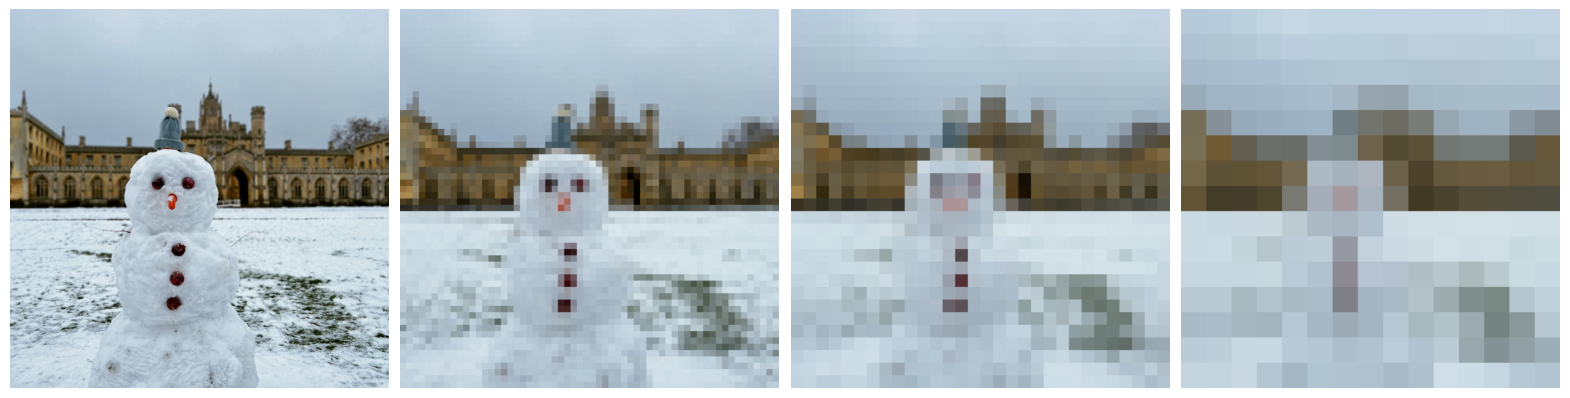
\includegraphics[width=\linewidth]{Images/pixelate_image_snowman.png}

   \caption{A pixel, a picture element, is the smallest unit of a rendered image. Displaying an image with fewer pixels causes losses in details as one pixel starts covering a larger area in the 3D scene.}
   \label{fig:colour-approximate}
\end{figure}

Let's consider the display of a sphere on a computer screen. We apply a grid on the sphere to represent pixels. Some pixels have a constant colour of the object, while some are blank. On the other hand, some pixels include different shades of the object colour or some are half-overlapped with the sphere. The question here is how to fill the pixels with mixed colours. 

hey
In a simple case where we only have a single colour with a blank background, we can subdivide this pixel into sub-pixels and count the number of pixels that belong to the object and the background. Later, the colour of the corresponding pixel can be approximated by taking the weighted average between the background and object colour. For instance, Figure \ref{fig:display-grid} shows the display of a sphere with grids symbolising pixels. The sub-pixels on the right can be counted to compute the colour of the corresponding large pixel. The generalized implementation of this approach can be seen in Figure \ref{fig:colour-approximate}, where I computed the mean value with a sliding window of different sizes (50, 100 and 200 in order, for image size of 3024 x 4032).

\begin{figure}
  \centering
  % \fbox{\rule{0pt}{2in} \rule{0.9\linewidth}{0pt}}
   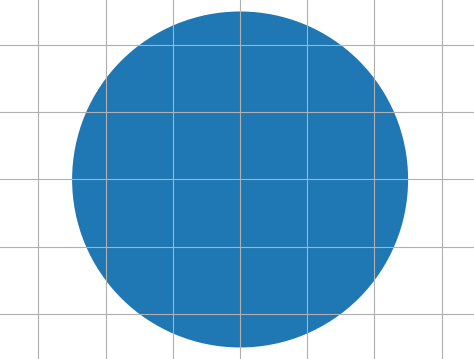
\includegraphics[width=0.4\linewidth]{Images/grid_circle.png}
    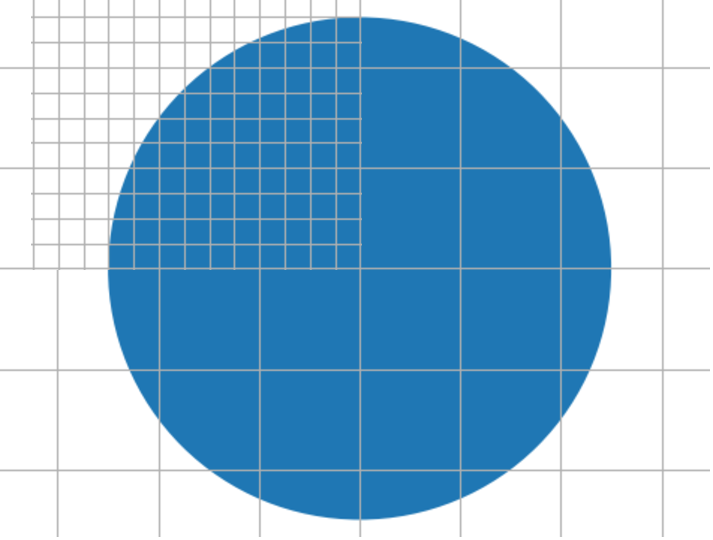
\includegraphics[width=0.4\linewidth]{Images/merged_grid_circle2-crop.pdf}

   \caption{To compute the colour of a pixel with variations, it is common to divide the pixel into sub-pixels and take the weighted average of each sub-pixel.}
   \label{fig:display-grid}
\end{figure}


\begin{wrapfigure}{l}{8.5cm}
\includegraphics[width=0.9\linewidth]{Images/colourspace.png}
\caption{Comparison of different colour gamuts. Image from [Schewe and Fraser, 2007].}\label{fig:colour-gamut}
    
\end{wrapfigure} 

Another approach would be to increase the resolution of an image, defined by the number of pixels per image. Nonetheless, this improvement is constrained by the screen’s resolution. As we endeavour to simulate the real world, the discretization process remains a part of this virtual representation. Furthermore, it is not merely the surface of objects that requires discretization; the colour of each pixel must also be pieced into bits for digital storage. In other words, the number of colours we can display is restricted by the number of bits used for colour encoding. 

In the developing stages of computing, the brightness of each pixel was represented by a single bit: a value of one for white and zero for black. These days, one of the most commonly used colour spaces, standard RGB space (sRGB), encodes each colour with 8 bits, requiring $8 * 3 = 24$ bits per pixel. Figure \ref{fig:colour-gamut} compares different colour spaces for the range of available colours in their space, known as colour gamut. Here, the question about pixel colour computation changes to how we can display a colour that is unavailable in a colour space. This problem is known as colour quantisation. The solution would be again approximating the desired colour with the closest matching colour available in the space/palette.

% \begin{figure}
%   \centering
% \caption{Comparison of different colour gamuts \cite{schewe2007colour}}\label{fig:colour-gamut}
%     \includegraphics[width=0.44\linewidth]{Images/colourspace.png}
% \end{figure} 
% %-----------------


The issue with colour quantization is that few colour samples might not accurately represent the continuous colour spectrum, causing discrete steps, bands, between the colour samples (see Figure \ref{fig:colour-band}). Luckily, the current image formats allow 24 (sRGB) / 32 (RGBA) bits to encode colours, displaying more than 16 million distinct colours, reducing the colour banding effect significantly. Nevertheless, the representation of continuous signals in the virtual environment remains limited due to the discretization of the data with bits for storage in a computer.

Another problem to consider is aliasing, which occurs when the sampling frequency for discretization is lower than twice the continuous signal bandwidth (Nyquist Theorem). The range of frequencies you can capture in a scene depends on the image resolution or pixel size. For instance, if an object is too far from the image plane, its projection can become smaller than the pixel size, for which we end up seeing the object as a dot.



\begin{figure}
  \centering
    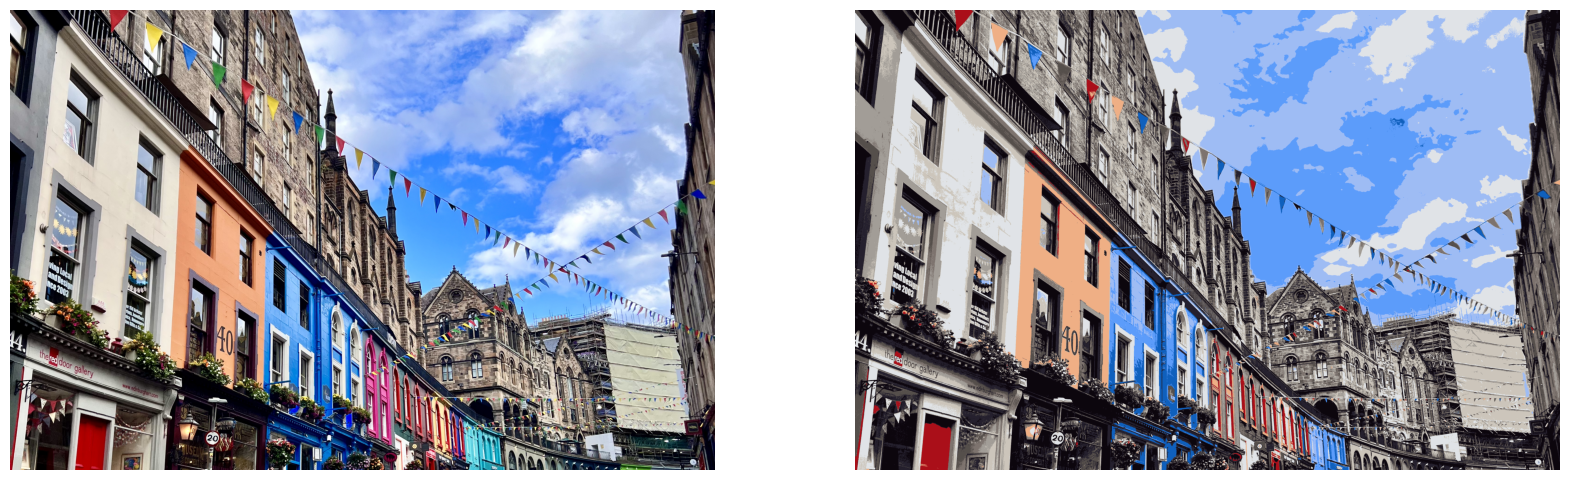
\includegraphics[width=0.9\linewidth]{Images/colour_quantization.png}

    \caption{When a colour is represented with too few bits, the transition between colours appears as discrete steps, known as colour banding (right).}\label{fig:colour-band}
\end{figure} 


Note that the pixel-based display discussed above is called raster graphics or raster display. It lays the image onto a two-dimensional array of pixels with a grid of x and y coordinates on a display space. Here, zoom-in does not bring any additional details due to limitations of the image and screen resolution. On the other hand, vector graphics stores the shape of objects with mathematical expressions instead of pixel values, offering flexibility with the resolution as the shape of the objects is computed based on the desired resolution.

\subsection{3D scene components}

A 3D scene consists of objects of different sizes, shapes, and appearances. To render an image of a scene, we first need a viewpoint represented by a camera. This mimics the case in the human visual system (HVS), where we look at a scene from a certain point, and the image of the scene appears in our retina. Without any light, all scene components appear dark. Therefore, light is a crucial aspect of the scene description. Another aspect is geometry, which defines the shape of the objects. Geometry, camera and light are three essential components of a 3D scene. While rendering a scene in a 3D software platform, such as Blender or Maya, a scene file contains all this information along with material/texture details. The light-material interaction defines the appearance, which this thesis focuses on. Before delving into the details of what appearance is in computer graphics, I will briefly review geometry as it builds up a baseline for appearance representations.

\begin{figure}
  \centering
  % \fbox{\rule{0pt}{2in} \rule{0.9\linewidth}{0pt}}
   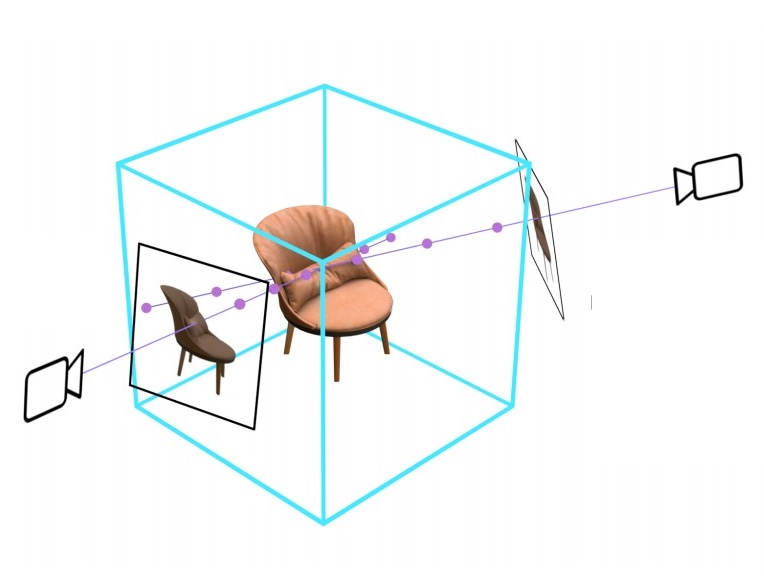
\includegraphics[width=0.7\linewidth]{Images/scene_with_camera.jpg}
   \caption{Rendering an image of a 3D scene requires lighting, viewpoint (camera) and geometry. Image from [Boss et al., 2021].}
   \label{fig:teaser}
\end{figure}


\paragraph{Geometry.} In the real world, what differentiates the state of the objects is the density of the matter the objects consist of. For instance, clouds are made up of loosely connected molecules with large holes in between. Wood and metal are densely composed with little space between the molecules. On the other hand, computer graphics assumes that objects are either solid or not, keeping things simple since the external shape of an object is what matters at the end. 


In general, the shape of an object is represented with 3D points in computers' memory, with $x$, $y$, $z$ axes defined in the Cartesian coordinate system. The surface (a polygon) can be constructed by connecting multiple points on the same plane (co-planar). The simplest polygon we can create is a triangle. Triangles are widely used because of their simplicity and efficiency, which led to the development of multiple efficient algorithms to compute the intersection of a triangle with a line. In case surfaces are defined by many points, it is common to divide them into multiple triangles, known as triangulation. Although the real-world objects are not naturally polygonal, this simplification helps efficient rendering and digital representation.

\begin{figure}
  \centering
  % \fbox{\rule{0pt}{2in} \rule{0.9\linewidth}{0pt}}
   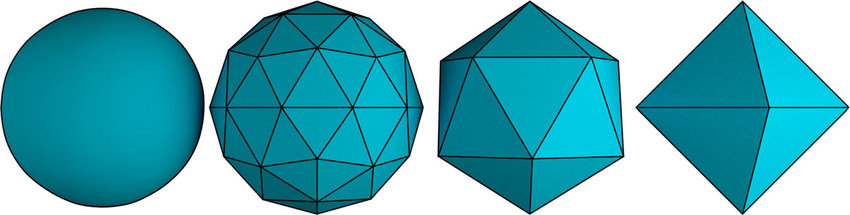
\includegraphics[width=0.7\linewidth]{Images/Triangulation-of-surfaces-Any-curved-surface-in-this-case-a-sphere-can-be-approximated.png}
   \caption{Triangulation of surfaces is a commonly used method in computer graphics to define the shape of objects. It allows the creation of complex shapes. Increasing the number of triangles also increases the resolution of the shape that leads to smoother surface representations. Image taken from [Broeren et al., 2019].}
   \label{fig:triangulation}
\end{figure}

One might wonder how triangulation handles the reconstruction of smooth surfaces. It is indeed not not optimal solution. However, considering a smooth curve, we can approximate it by taking a few points (samples) on the curve and connecting them with straight lines (segments). To enhance the resolution, we can take more samples, that is, reduce the size of the segments. By applying this to smooth surfaces, we can increase the number of triangles (Figure \ref{fig:triangulation}) that will eventually increase the rendering time. Converting a smooth surface to triangular mesh is known as tesselation.

Returning to the early discussion on discretization, computer graphics only approximates the shape of real-world continuous objects with discrete data. Since the ultimate goal is to display these shapes on a screen that also operates with discrete data, one well-known approach to conceal the triangular look of a surface is to keep the size of the triangles smaller than the pixel size. This approach has been used widely in professional rendering programs, such as Pixar's RenderMan, and has recently taken its place in real-time applications.

Ray tracing algorithms, which HyperBRDF is built on, do not necessarily need a polygonal representation of objects. Ray tracing computes the intersection point of a ray (a straight line) with the object surface, which can be found either with a geometric or an algebraic solution. The algebraic solution becomes feasible when the surfaces are defined by mathematical equations, known as implicit/algebraic surfaces. A ray equation, essentially a line equation, and the mathematical equation for the surface of an object give us a system of linear equations for which a solution exists if the ray and the object intersect.

 Although geometry can be defined by various methods, such as meshes, NURBS, subdivision surfaces, implicit surfaces, etc, this section only discusses polygonal mesh representation. Triangle is the most common rendering primitive used in ray tracing and on modern GPUs. Since the support of only one primitive is preferred due to simplicity and efficiency, most 3D platforms first convert geometry to triangular meshes before rendering.
 
\subsection{Photo-realistic rendering}
There are different approaches to render an image of a scene. Whichever rendering method we choose, we should expect the same image as the output. In photo-realistic rendering, which is often the most desired, the expectation from a rendered image is to look the same as how our eyes perceive the scene. In other words, the image should look like a "photograph". Achieving such photo-realism requires us to understand two main aspects of our visual system: 1) geometric construction of the shapes with respect to other objects, 2) the physics laws behind appearance. More specifically, photo-realistic rendering focuses on simulating the behaviour of light throughout its propagation and interaction with matter.

\paragraph{Perspective projection and visibility.}

The human visual system is inherently an optical system that converges light rays reflected from objects to a focal point. Following the geometry, our eyes perceive objects that are further away smaller than the closer objects of the same size. In other words, objects get smaller in the rendered image in our retina as they move away from our eyes, known as the foreshortening effect. The lens systems in cameras already replicate this effect, and photo-realistic rendering also aims to achieve the foreshortening effect along with simulating the physics laws for appearance.  

To achieve foreshortening effect, imagine we have a canvas or an image plane between the eye and the object. By tracing the lines from the eye to the corners of the objects, we can find the location of the projected corners (points) on the image plane (perspective projection). We can then draw the objects' edges on the image plane to complete the look. However, this look is unlikely to be photo-realistic as we haven't figured what edges are visible from the viewpoint. For instance, if it were an opaque cube, then the back sides would remain hidden behind the front sides. Therefore, rendering involves computations for both the visibility problem and the perspective projection. 

\begin{figure}[ht]
  \centering
  % \fbox{\rule{0pt}{2in} \rule{0.9\linewidth}{0pt}}
   \includegraphics[width=0.6\linewidth]{Images/perspective_projection.png}
   \caption{Perspective projection mimics the foreshortening effect our visual system creates while observing a scene. The image plane/canvas includes the 2D projections of the visible objects within the view frustum.}
   \label{fig:perspective_projection}
\end{figure}


We can project a 3D scene onto a flat surface in different ways. For instance, in artistic drawing, perspective projection can include multiple focal points (Figure \ref{fig:artistic_drawing}). However, computer graphics generally assumes one-point perspective as it mimics our visual system as well as cameras. In this approach, the line of sight, the line from the eye perpendicular to the canvas, passes through the center of the canvas. The view frustum is the region of the scene projected onto the canvas. The lines passing through the corners of the canvas forms the frustum base (Figure \ref{fig:perspective_projection}). Here, we can change the size of the canvas, which results in the change of the frustum size and, consequently, the visible region of the scene. This resembles the techniques in photography where changing the focal length of the camera lenses adjusts the field of view.

\begin{figure}[ht]
  \centering
  % \fbox{\rule{0pt}{2in} \rule{0.9\linewidth}{0pt}}
   \includegraphics[width=0.4\linewidth, height=4.5cm]{Images/single_point_perspective.png}
    \includegraphics[width=0.4\linewidth, height=4.5cm]{Images/two_points_perspective.png}

   \caption{Single-point vs two-point perspective. Computer graphics mimics our visual system, focusing on single-point projection. However, multi-point perspective is widely explored in artistic drawing.}
   \label{fig:artistic_drawing}
\end{figure}


% \paragraph{Visibility problem}
The visibility problem occurs when some parts of the scene are not visible from a known viewpoint. For instance, if we only project the corners of an object and draw the edges, then some corners that shouldn't be visible from the known viewpoint will be included in the rendered image. Furthermore, some objects will be occluded by others. Computer graphics tackles the visibility problem in two ways: rasterisation and ray tracing. I will not go into the details of these algorithms as this is beyond the focus of this thesis.

% In this section, I will mostly focus on ray tracing as HyperBRDF is designed for such renderers.Photo-realistic rendering aims to project or flatten a 3D scene onto an image plane that lies between the scene and the camera position or the viewpoint. Mimicking our visual system, we first apply perspective projection via similarity formula in geometry and then decide which points are visible from the viewpoint. Some will be indeed occluded by other objects or the front sides. 

\paragraph{Appearance.}
Perspective projection and visibility only project the size and shape of the scene realistically without any consideration for appearance, such as the colour, texture, brightness, etc. We can only perceive an object if the light bounces off its surface. Therefore, appearance involves light-matter interactions, where the light travels in a ray form in space and gets absorbed or reflected when it interacts with the surface of an object. Different light sources, such as the sun or light bulbs, can emit light. After the light bounces off a surface, it continues its journey until it either reaches our eyes, where it is converted to electrical signals or another surface where the interaction steps repeat.

\begin{wrapfigure}{l}{4.8cm}
  \centering
  % \fbox{\rule{0pt}{2in} \rule{0.9\linewidth}{0pt}}
   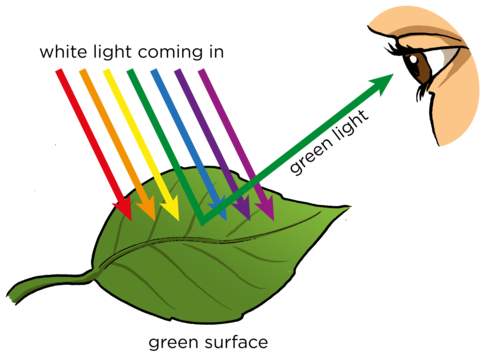
\includegraphics[width=\linewidth]{Images/object-colour.png}
   \caption{The reflected light from the surface of an object defines its colour. Image from \href{http://www.mstworkbooks.co.za/natural-sciences/gr8/images/gr8ec04-gd-0027.png}{website link}.}
   \label{fig:object-colour}
\end{wrapfigure}

The colour of an object is defined by the mixture of the reflected light colours (Figure \ref{fig:object-colour}). The light colour is a continuous spectrum with the visible light lying between 380 to 700 nanometers in wavelength. For instance, a leaf reflects green light while absorbing the remaining visible spectrum. Another example would be a black object that absorbs all visible lights or a white object that reflects them all.

At the object level, reflection can be considered a mirror-like look, where the light turns around the normal to the surface at the point of contact. The outgoing direction becomes the reflected version of the incoming one. Microscopic level interactions are more complex with light bouncing off in random directions, known as scattering. Computing the photon-atom interactions is indeed impractical. Therefore, computer graphics researchers have developed mathematical models to simulate the light-matter interactions at the microscopic level. I will discuss them later in this chapter. Section \ref{hyperbrdf-RW} will also compare HyperBRDF with such mathematical formulas. Here, I will overview some of the well-known shading and lighting effects:

\begin{wrapfigure}{r}{4.8cm}
\includegraphics[width=\linewidth]{Images/rough_river_surface_reflection.png}
\caption{The ripples on the water's surface cause a blurred image of the bridge, acting as a rough surface.}\label{fig:water_reflection}
\end{wrapfigure}  

\textbf{\textit{Reflection}} occurs when light interacts with mirror-like objects that change the direction of light in the reverse direction with the same angle reflected around the point of contact. The incoming light, also known as the incident light, turns around the normal and leaves the surface in the reflected/outgoing direction (Figure \ref{fig:microfacet} - right). Metals, such as silver and aluminium are considered materials with high reflectivity. The surface of the water or glass also creates reflection, but their reflectivity is considerably lower.

\textbf{\textit{Specular reflection}} appears when the surface is not perfectly smooth, and its roughness causes lights to bounce off in different directions. Consider a rough surface at the microscopic level having many microfacets looking in slightly different directions. The complex nature of the material surface then reflects the lights at a microfacet level, each microfacet acting as a mirror (Figure \ref{fig:microfacet}). The overall outgoing light becomes the combination of each of these reflections, known as specular or glossy reflection. Most often, these microfacets are not visible to our eyes akin to smooth surface appearance. The deviation of lights from the mirror direction depends on how rough the surface is, that is, how varied the facet orientations are with respect to a smooth surface. More microfacets with higher variance in orientations will lead to greater divergence from the mirror angle, enlarging the glossy region of the surface. Here, roughness and glossiness are used antonymous to describe the specularity of a material. This kind of reflection often leads to blurred or deformed images, as shown in Figure \ref{fig:water_reflection}. 



\begin{figure}
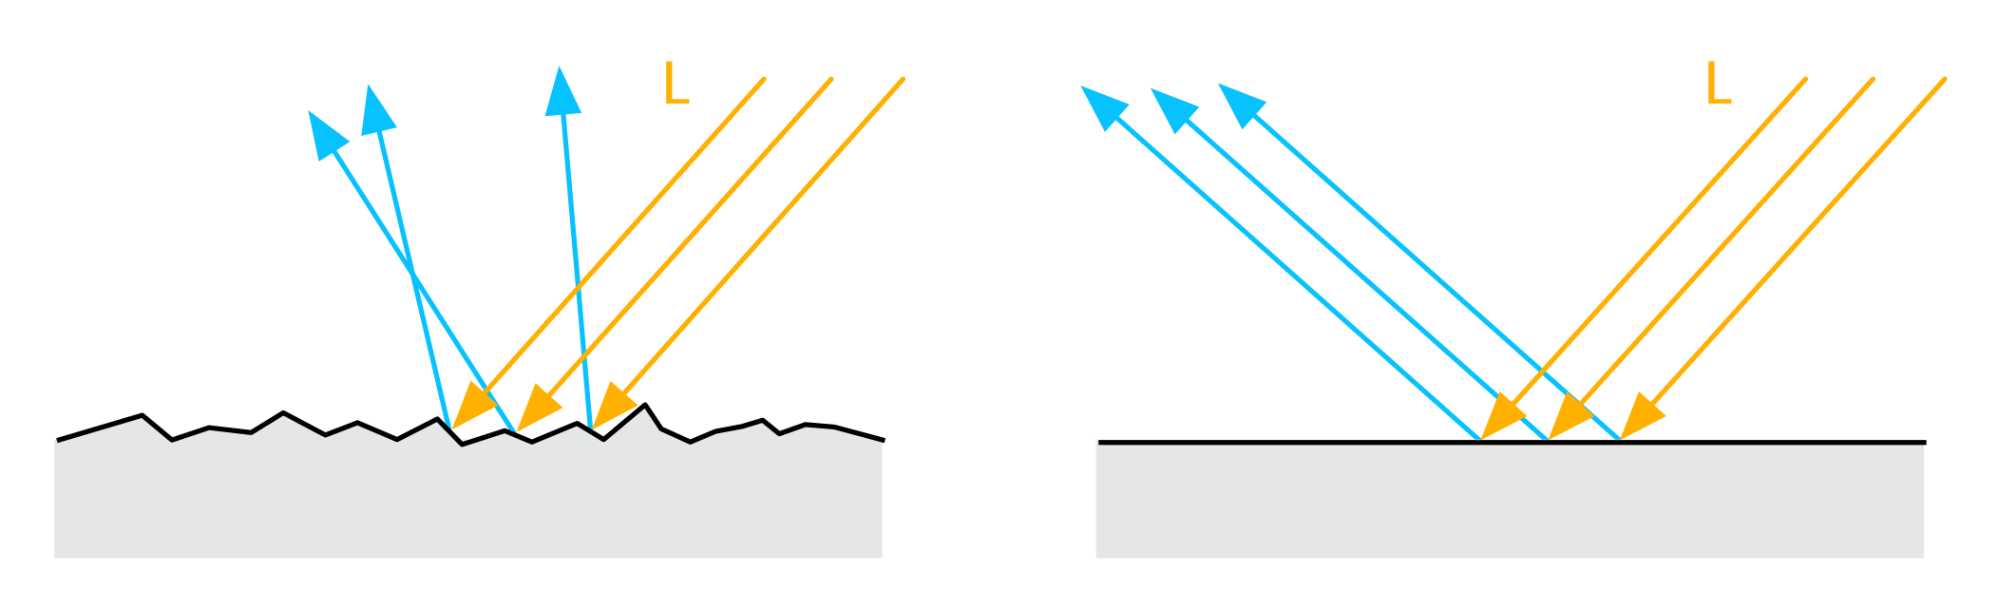
\includegraphics[width=0.9\linewidth]{Images/diagram_microfacet.png}
\caption{Reflection on a surface with microfacets vs smooth surface. Image from [Guy and Agopian, 2024]}\label{fig:microfacet}
\end{figure} 

% \begin{figure}
%   \centering
%   % \fbox{\rule{0pt}{2in} \rule{0.9\linewidth}{0pt}}
%    \includegraphics[width=0.5\linewidth]{Images/rough_river_surface_reflection.png}
%    \caption{The ripples on the surface of the water causes a blurred image of the bridge, acting like a rough surface.}
%    \label{fig:water_reflection}
% \end{figure}


\textbf{\textit{Diffuse reflection}} is the reflection that we observe when the incident lights are so scattered that they reflect in random directions, equally spread. Diffuse surfaces are either extremely rough or composed of tiny structures where the light gets trapped, reflected and refracted multiple times before leaving the surface (Figure \ref{fig:diffuse-scattering}). The outgoing direction becomes independent from the incident direction due to the large number of internal reflections underneath the surface. This randomness results in the object appearing equally bright in all viewing directions. 

\begin{wrapfigure}{l}{6.5cm}
  \centering
  % \fbox{\rule{0pt}{2in} \rule{0.9\linewidth}{0pt}}
   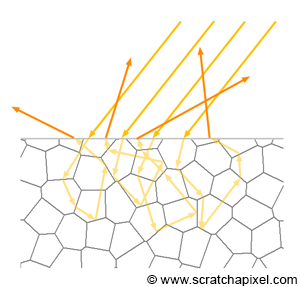
\includegraphics[width=0.5\linewidth]{Images/shad-diffuse1.png}
   \caption{Diffuse surfaces often have complex internal structures that cause the light to be reflected multiple times underneath the surface.}
   \label{fig:diffuse-scattering}
\end{wrapfigure}


\begin{figure}[ht]
  \centering
  % \fbox{\rule{0pt}{2in} \rule{0.9\linewidth}{0pt}}
   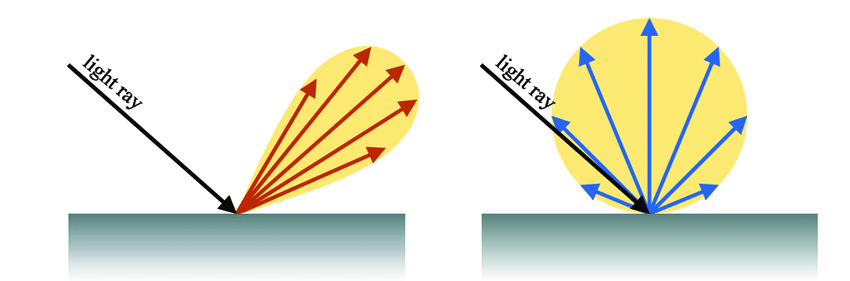
\includegraphics[width=0.7\linewidth]{Images/Differences-between-the-specular-and-diffuse-reflections-specuclar-reflections-occur-on.png}
   \caption{Specular vs diffuse reflection. Diffuse surfaces cause rays to scatter randomly, brightening the object equally in all viewing directions. Specular reflection is, on the other hand, view-dependent, reflected rays concentrated around the mirror reflection. Image from [Park and Baek, 2021].}
   \label{fig:specularvsdiffuse}
\end{figure}

Diffuse surfaces, also known as Lambertian or matte surfaces, differ from specular ones in that diffuse materials are often formed of multiple internal pieces that trap the light, causing the light's outgoing direction to become independent from the viewpoint. Specular ones, on the other hand, are modelled with microfacets that reflect the light rays around the mirror angle, remaining correlated with the incoming direction. As diffuse reflections are view-independent, the brightness of a diffuse surface remains consistent across all viewing angles (Figure \ref{fig:specularvsdiffuse}). This distinction can be observed when looking at real-world materials, observing how their brightness changes when we move around, changing our viewpoint.


Some other lighting and shading effects include transparency, subsurface scattering, indirect lighting and shadows. When light contacts a transparent object, such as glass or water, it bends and passes through the surface in a different direction, which can be computed using Snell's Law. Subsurface scattering, also known as translucency, occurs when light travels within the object, leaving the object at a different point and direction. Wax, marble or thin layers of skin are considered as translucent objects. Indirect lighting is the result of the light being reflected from other surfaces, illuminating the object without any direct light from the light source. Lastly, shadows are dark regions due to light being blocked by an object. 

The appearance of a scene depends on how light interacts with an object and the path light travels through. All the aforementioned effects contribute to appearance. Some effects, such as reflection, specularity, diffuse, transparency and subsurface scattering, relate to material properties. They affect shading, the appearance of an object. Other effects (shadows and indirect lighting) depend on the light's journey (light transport), that is, how much light the object gets after the light interacts with multiple surfaces. 

Shading is concerned with the interaction of light with the material. Light transport tracks the light's path throughout its journey while it bounces off surfaces. It takes into account the obstructions, changes of reflections, etc. In the real world, the two are not differentiated as they determine the appearance together. However, computer graphics keep these two distinct for efficient and practical computations. It is worth mentioning that simulating light-matter interactions is more challenging than tracking the light path. The latter is more straightforward, while the former requires simplifications for the material representations.



\paragraph{Ray tracing - Light transport simulation.}

Light starts its journey from a light source and travels in a straight line, bouncing off surfaces. Following this path to simulate the light is known as forward tracing. However, not all rays emitted from a source will reach the eye/camera. Considering their size, most rays are unlikely to contribute to our view of the scene, travelling in different directions. As it is highly impractical to trace all rays, including those not contributing to our view, ray tracing algorithms trace the rays from the eye to the light source in the reverse direction for efficient computations (backward tracing).

The simulation starts with shooting rays from the virtual camera to the light source for each pixel on an image plane (Figure \ref{fig:raytracing}). Here, the view ray, also known as the primary or camera ray, passes through the centre of a pixel. The colour of that pixel is computed by the shading algorithms that define the light-material interactions. Let's imagine we shoot a ray that encounters an object on its way to the light source. The intersection point can be found by equating the mathematical equations defining the ray (a line) and the object. If a solution exists, then the object and the ray intersect. Once we obtain the intersection point with the object, we can shoot shadow rays from that point to the light source to compute the diffuse and specular reflections at the corresponding point. If the shadow ray encounters another object before reaching the light source,  the intersection point remains in the shadow of the other object. Furthermore, the ray can be absorbed, reflected or refracted based on the material properties. In the case of reflection, new rays can be spawned to compute the contribution of the reflection to the colour of the object.


\begin{figure}
  \centering
   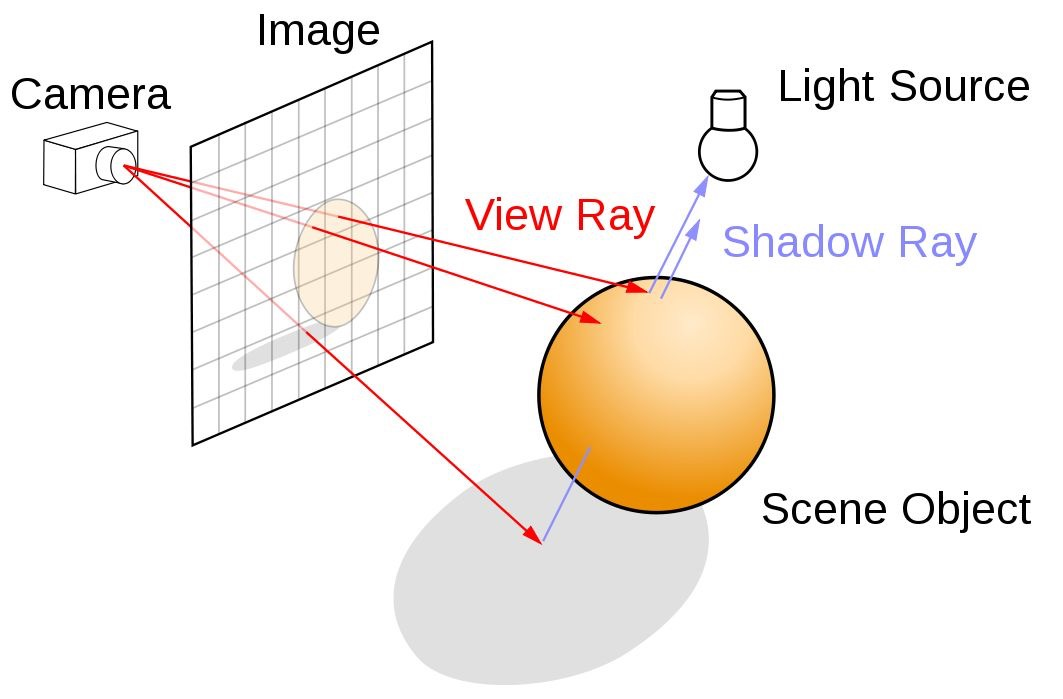
\includegraphics[width=0.5\linewidth]{Images/ray-tracing-image-1.jpg}
   \caption{Ray tracing simulate the light's journey to compute the colour of each pixel on the rendered image.Image from [Henrik, 2008].}
   \label{fig:raytracing}
\end{figure}

Shooting only one ray per pixel can cause issues, such as jagged edges or missing tiny objects. To alleviate such issues, we can shoot multiple rays in a sub-pixel grid or in a random setting. However, this increases the render time because of the large number of computations required to trace the rays. This brings us to the trade-off between the render time and the accuracy of the rendered image. This trade-off often leads to different applications, such as virtual effects in the film industry requiring high accuracy with longer render time and real-time AR/VR applications with fast rendering but relatively low quality.

Ray tracing is a computationally expensive rendering technique that simulates the light transport realistically, following the laws of physics. Unlike rasterization, ray tracing does not deal with perspective projection or visibility explicitly or separately. Instead, it simulates both naturally by computing the intersection points of the ray with objects. Here, I explained the basics of the algorithm, which has advanced in recent years with intensive versions known as path tracing. 

\subsection{Shaders and BRDF}

Shading is the process of computing the colour of objects seen from the camera's viewpoint. Earlier, we discussed that achieving photorealism involves two main steps:  visibility along with perspective projection and shading. If we are to achieve photorealism, shading should reproduce the appearance of a scene so realistically that our eyes perceive the rendered image the same as the real word. A photorealistic image should look like a photograph of the same scene taken from the same viewpoint. 

Appearance is, in principle, the by-product of illumination and object properties. As the scene gets more light, objects are likely to appear brighter. Object properties that determine the appearance are reflectivity, which defines light-material interactions, and the geometric construction, i.e., orientation. The object colour we perceive is the mixture of light rays reflected off the surface. Objects often do not emit light but are lit by light sources emitting rays. This emitted light hits the surface of the object, some of which is later reflected off the surface and reaches our eyes, creating the object's colour. This type of lighting is known as direct lighting since the reflected light directly comes to our eyes after visiting the object. Indirect illumination occurs when an object gets some light reflected off other objects. Light can bounce off multiple surfaces, even infinitely many, before reaching our eyes.

Let's return to the discussion on lighting and shading effects we observe in the real world. We mentioned that what differentiates the objects with mirror-like,  specular and diffuse surfaces is the way they reflect the incoming light. A diffuse or Lambertian surface randomly spreads the incident light, looking equally bright in all viewing directions. Mirror-like objects reflect the ray around the point of contact, while specular surfaces distribute the light around the mirror direction. In the case of mirror-like or specular surfaces, the objects wouldn't be visible if our viewing direction is far from the mirror direction. Although we clearly distinguish different types of surfaces in computer graphics, real-world surfaces do not necessarily show only one kind of reflection.


Most real-world objects can exhibit both diffuse and specular reflections at the same time. This can happen either because the object is composed of multiple materials with different reflectivities joined together, or it has multiple layers of materials added on top of each other, as in the skin layers. Putting them together, we can define the overall appearance as the weighted sum of diffuse and specular components: 
\begin{equation}
I = k_d * I_d + k_s * I_s
\end{equation}
where $I$ is the total intensity of the light reflected by the surface at the point of contact, $I_d$ and $I_s$  are diffuse and specular intensities, and $k_d$ and $k_s$ are their corresponding coefficients. Here, we oversimplify the representation, neglecting shadows and interaction between objects.



\begin{wrapfigure}{l}{7.5cm}
  \centering
  % \fbox{\rule{0pt}{2in} \rule{0.9\linewidth}{0pt}}
   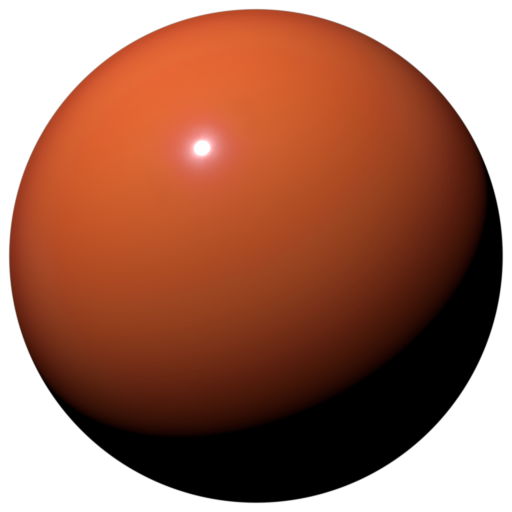
\includegraphics[width=0.5\linewidth]{Images/specular+diffuse.png}
   \caption{A material composed of both specular and diffuse components, lit by a point light source. The specular highlight (white circle) is centered around the light source direction. The material is specular-maroon-phenolic from MERL dataset \cite{Matusik2003jul}.}
   \label{fig:diffuse+spec}
\end{wrapfigure}


The diffuse shading can be computed based on the angle between the normalized incident light direction $L$ and the normal to the surface $N$:
\begin{equation}
I_d = I_l \, k_d \cos(\theta) = I_l \, k_d \, (N . L)
\end{equation}
where $I_l$ is the intensity of the light source. Note that the lights with different colours can have different $I_l$ and $k_d$. Also, $\cos(\theta) < 0$ indicates that the light remains behind the surface, not contributing to the brightness on the visible side. The effect of $\cos$ term is visible in Figure \ref{fig:diffuse+spec}, where the diffuse intensity gets dimmer as the points on the surface gets further away from the point of contact (specular highlight). 

\begin{figure}[ht]
  \centering
  % \fbox{\rule{0pt}{2in} \rule{0.9\linewidth}{0pt}}
   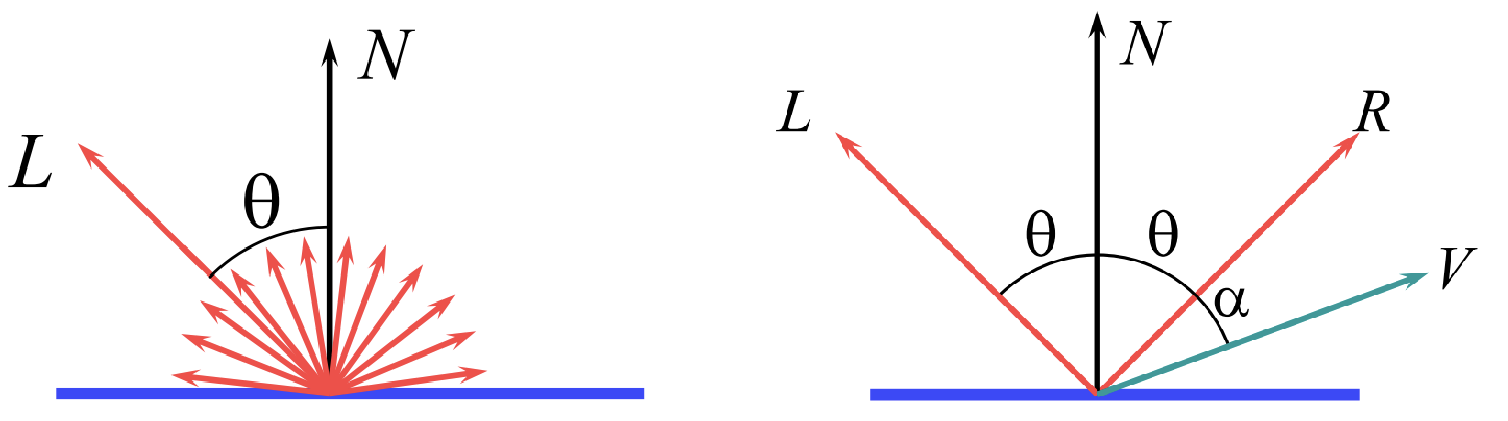
\includegraphics[width=0.5\linewidth]{Images/diffuse+specular+angle.pdf}
   \caption{Diffuse and specular reflections.. Figures from [Mantiuk, 2022]}
   \label{fig:diffuse-spec-angle}
\end{figure}

Furthermore, the specular term can be approximated by:
\begin{equation}
I_s = I_l \, k_s \, \cos^n(\alpha) = I_l \, k_s \, (R . V)^n 
\end{equation}
where $R$ is the mirror reflection, $V$ is the viewing direction, and $n$ is an ad-hoc roughness coefficient (Figure \ref{fig:diffuse-spec-angle}).


We mentioned that the consideration of only diffuse and specular reflections ignores indirect lighting, which can be compensated by adding an additional constant term, $I_a * k_a$, known as ambient illumination. The overall shading then becomes:

\begin{equation}
I = I_a * k_a + \sum_i \, I_i \, k_d \, (N . L) + \sum_i \, I_i \, k_s \, (R_i . V)^n
\label{eq:Phong-eq}
\end{equation}

This mathematical model is known as the Phong shading model, a well-known shading model used for decades in computer graphics. The simplified specular reflection term was introduced by Phong in 1998 \cite{phong1998illumination}. This model does not take into account the shadows, requiring an additional ray tracing or shadow mapping for the simulation of shadows. It also considers the light sources infinitely far from the surface, ensuring the lighting direction $L$ remains the same across the surface.

Modelling light-material interactions is extremely complex due to the nature of materials. Hence, computer graphics researchers have developed mathematical models to approximate the function defining the reflectance of a material surface. This function is known as the Bidirectional Reflectance Distribution Function (BRDF). The Phong shading model is one of the most popular BRDF approximation models due to its simplicity. Some other mathematical models include Cook-Torrance~\cite{cooktorrance1982}, Ward~\cite{ward1992} and GGX~\cite{walter2007microfacet}, with GGX being the most widely used approximation for its realistic results. I will compare HyperBRDF with GGX results in Chapter \ref{ch:HyperBRDF}.

Before going into the details of BRDF, let's examine the effect of the roughness term in the Phong model:

\begin{figure}[ht]
  \centering
  % \fbox{\rule{0pt}{2in} \rule{0.9\linewidth}{0pt}}
   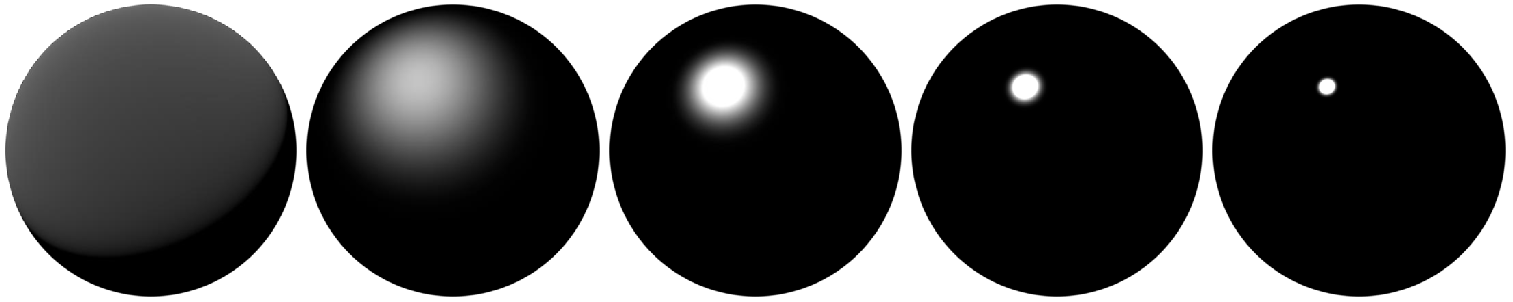
\includegraphics[width=\linewidth]{Images/Phong-roughness-coeff.pdf}
   \caption{Phong shading model implementation with decreasing roughness/increasing glossiness from left to right.}
   \label{fig:phong-roughness}
\end{figure}

\begin{wrapfigure}{l}{6cm}
  \centering
  % \fbox{\rule{0pt}{2in} \rule{0.9\linewidth}{0pt}}
   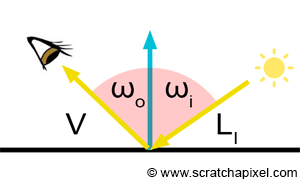
\includegraphics[width=\linewidth]{Images/shad2-brdfdir}
   \caption{BRDF depends on the incident light and viewing direction.}
   \label{fig:brdf}
\end{wrapfigure}
The rougher the material surface is, the more matte the object appears. As we decrease its roughness by increasing the value $n$, the specular highlight becomes a mirror-like reflection around the point of contact. 


\paragraph{BRDF.} 
Looking at Eqn. \ref{eq:Phong-eq}, we observe that the appearance/shading depends on two variables: incoming light direction for diffuse and specular terms and viewing direction for specular only. Therefore, we can generalise this function as a function with two parameters as  $f_R(\omega_o, \omega_i)$, where  $\omega_o$ is the angle between the surface normal and viewing direction and the surface normal and the light direction (Figure \ref{fig:brdf}). This function, known as BRDF, gives us the amount of light reflected in the viewing direction when the surface is lit in the incoming light direction.

The mathematical formulations, such as Phong or GGX, approximate $BRDF(\omega_o, \omega_i)$s of real-world materials with simplifying assumptions on their nature. For instance, some models are designed to simulate only certain material types (Oren-Nayar model for Moon's BRDF). Some models follow the principle of optics or are designed empirically (Phong). Fitting to measured BRDF values is another alternative approach that recent neural network-based models, including HyperBRDF, are built upon.  

Comparing the mathematical approximations to real-world measurements helps us understand how accurate the BRDF model represents a real-world material. $BRDF(\omega_o, \omega_i)$ itself is defined based on the laws of physics and can be physically measured by some specialised hardware, such as gonioreflectometer. Cameras can also be used to measure the BRDF. For instance, the MERL dataset \cite{Matusik2003jul} is captured using a CCD camera. However, measuring the specular values can become a challenge with a camera capture due to the requirement of High Dynamic Range support. I will discuss such capture systems in Chapter \ref{ch:HyperBRDF}.

The BRDF is essentially a radiometric term with the usage in computer graphics for realistic simulations of light-material interactions. Hence, physically-based BRDFs hold the following properties:
\begin{itemize}
  \item positivity $f_R(\omega_o, \omega_i) \geq 0$, BRDF is positive across valid incoming and outgoing directions.
  \item Helmholtz reciprocity: $f_R(\omega_o, \omega_i) = f_R(\omega_i, \omega_o)$, The surface acts the same if the incoming and outgoing directions are switched.
  \item energy conservation. Unless the object emits light, the reflected light cannot be larger than the received one.
\end{itemize}


BRDF models should hold these physics-based properties to reproduce appearance realistically. In \citeauthor{Chenliang's paper} \cite{Chenliang's paper}, we discuss how these properties can be enforced in neural BRDF models. 

Rendering based on simulating the light's journey is computationally expensive. Therefore, a fast BRDF computation is an important consideration while choosing a model. For instance, Phong is a simple model that requires fewer computations. However, it is not energy-conserving. Recent mathematical models, such as GGX, have replaced Phong due to more accurate representations. Nevertheless, mathematical models still oversimplify the complex real-world BRDFs, constrained with a few parameters to tune. Therefore, recent work has started developing neural network-based approaches, which can offer higher capacity for the representation of highly-complex material appearance.

Lastly, we defined BRDF as the function of only two parameters, the incoming and outgoing directions, for which we assume that material properties remain the same across the whole surface. Complex real-world materials are composed of different substances, which results in showing various reflectivities at different points of contact. The Spatially Varying Bidirectional Reflectance Distribution Function (SVBRDF) can represent this behaviour with an additional location parameter ($f_R(\omega_o, \omega_i,  \vec{x})$). Furthermore, we assume that the reflected light leaves the surface at the point of contact, which unlikely occurs in translucent materials where we observe subsurface scattering. The Bidirectional Surface Scattering Reflectance Distribution Function (BSSRDF) represents such behaviour with additional parameters for both entry and exit locations ($f_R(\omega_o, \vec{x_o}, \omega_i,  \vec{x_i})$). For the rest of this thesis, I will only focus on BRDF representations with the assumptions mentioned here.

\subsection{Rendering Equation}

To conclude the rendering section, let's define the rendering equation used to reproduce the outgoing light in ray tracing algorithms for the realistic simulation of light-material interactions.:
\begin{equation}
L_o(\vec{x}, \omega_o) = L_e(\vec{x}, \omega_o)  +  \int_S^2 L_i(\vec{x}, \omega_i) \, f_{\vec{x}}(\omega_o,  \omega_i) \, \abs{w_i . N} d\omega_i
\label{eqn:rendering-eqn}
\end{equation}
Here, $L_o(\vec{x}, \omega_o) $ is the outgoing light at point $x$ in the direction of $\omega_o$, $L_e(\vec{x}, \omega_o)$ is the emitted light that represents the light sources, $L_i(\vec{x}, \omega_i) $ is the incoming light at point $x$ in the direction of $\omega_i$, $f_{\vec{x}}(\omega_o,  \omega_i)$ is the BRDF, and $\abs{w_i . N} = \cos(\theta_i)$ is the Lambert's cosine term.

The rendering equation gives the outgoing light at point $x$ for a given incident light direction with the known BRDF. Here, we can define the BRDF term in multiple ways, such as with mathematical models discussed earlier, with a neural network outputting the BRDF values when fed with the directions or with physical measurements captured with special instruments. 

\section{Machine learning}
This section gives an overview of the machine learning techniques I have utilised for the appearance manipulation techniques proposed in the following chapters. Machine learning techniques have become the state-of-the-art approach in most computer vision and graphics tasks due to their promising ability to learn. Especially the advances in the field with the introduction of deep learning that offers inherent nonlinearity have made these models ideal for tackling ill-posed image editing tasks that most often have $many$ solutions.

Starting with the learning process, I will first discuss the basics of machine learning, including multilayer perceptrons that will build the baseline for the machine-learning framework proposed in one-shot detail retouching. Later, I will discuss neural representations that offer the storage of the data in a novel neural network-based setup, which is very useful for the processing of visual data that usually lies in a complex high-dimensional space. The hypernetwork model I borrowed for the HyperBRDF model is a neural representation model generalizable to new data for reconstruction. Lastly, I will summarise diffusion models, specifically latent diffusion, for zero-shot transient attribute transfer.

\subsection{Foundations}
Machine learning (ML) is a subfield of artificial intelligence (AI) in which machines learn a task from data without explicit programming. ML algorithms, such as linear regression, decision trees or neural networks, define the procedure for the learning process. An ML model is the trained version of the algorithm used to make predictions or decisions. The model consists of internal variables (parameters) learned during the learning process, known as training. The model structure is called architecture, which can include tree nodes, neurons, layers, connections, etc.

\paragraph{Types of learning.} The data is the key to the success of any ML algorithm. Supervised learning methods use paired data, each training example including input data and its corresponding output (label). The model learns a mapping between the input and the output. Classification or image-to-image translation can be given as examples. Unsupervised learning approaches, such as clustering or dimensionality reduction, learn patterns from the data without any label. Some methods, semi-supervised methods, combine both labelled and unlabeled data. Lastly, reinforcement models learn the task with a feedback mechanism, including rewards and punishments. The ML algorithms I have utilised for my main approaches are based on supervised learning. Therefore, the rest of this section focuses on supervised learning.

\paragraph{Training.} During training, the model learns from a dataset, that is, updates its parameters to minimise the errors in predictions with a loss function. Training is an iterative method and starts with assigning initial values to model parameters. These initial values are, in general, chosen to be random. At each iteration, \textbf{epoch}, the parameters are adjusted with an optimiser, such as gradient descent or Adam, that reduces the errors in predictions. The errors are computed for each training example and averaged over the training dataset for the epoch loss. 

The large amount of data in the training set can make parameter updates slow and computationally expensive. Therefore, the dataset is often split into subsets, known as \textbf{batches}, and each batch is processed separately at each epoch. The \textbf{batch size} is the number of training examples in one batch. It affects the efficiency, the stability of the model updates and the convergence speed. The completion of one epoch means that the model passed through the entire dataset once. The number of batches multiplied by the batch size gives the total number of examples in the training dataset. For instance, if we have a dataset of 100,000 images and choose batch size 1000, we then process 100 batches to complete one epoch. 

\begin{wrapfigure}{r}{7cm}
  \centering
  % \fbox{\rule{0pt}{2in} \rule{0.9\linewidth}{0pt}}
   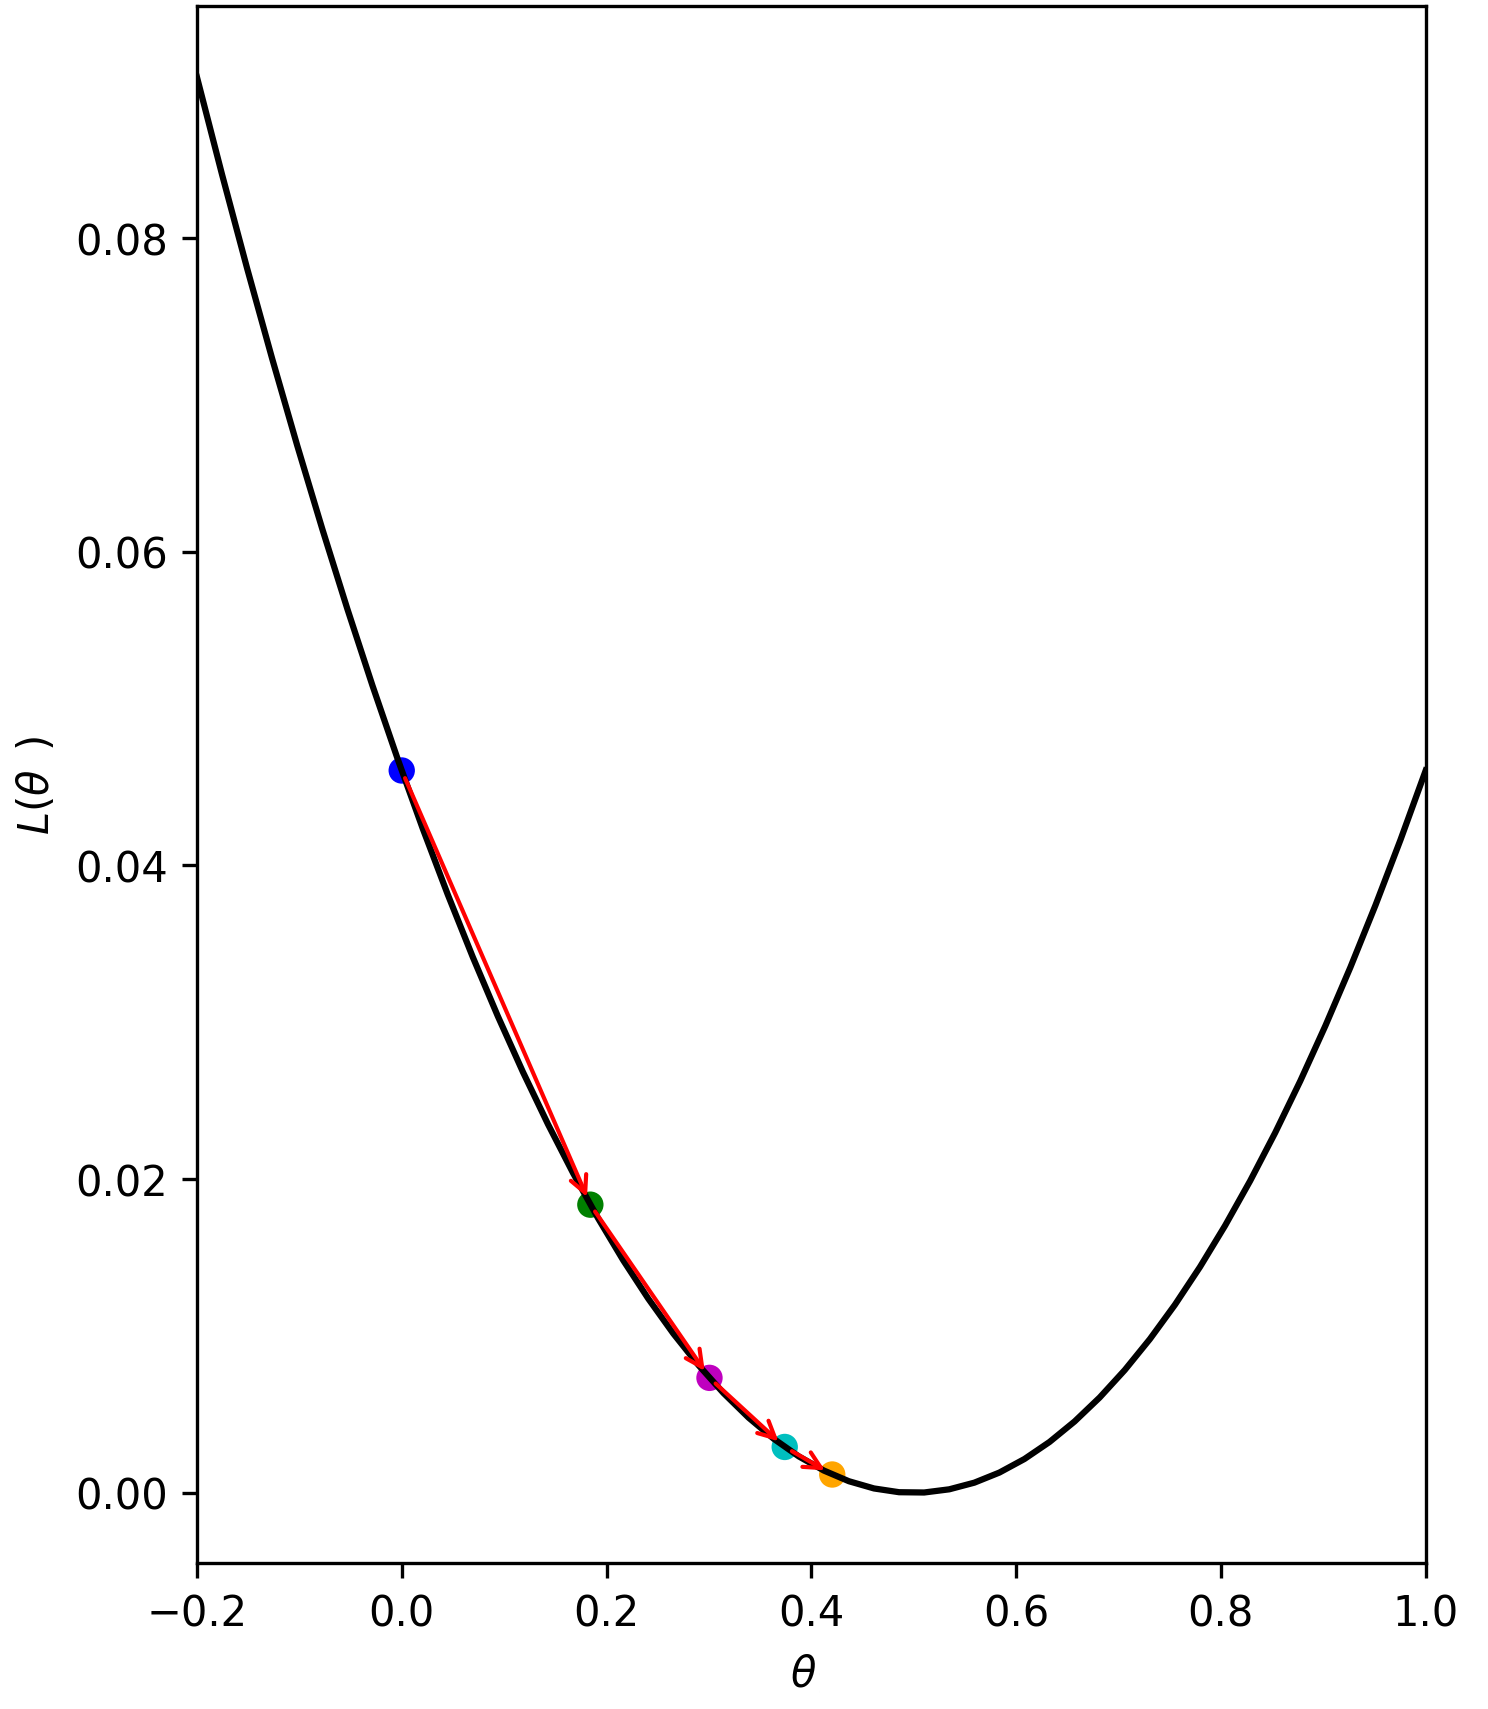
\includegraphics[width=\linewidth]{Images/gradient-descent.png}
   \caption{Gradient descent steps.}
   \label{fig:gradient-descent}
\end{wrapfigure}
The model parameters can be updated either after the entire dataset is passed through the model (\textbf{batch gradient descent}), or after each batch is processed (\textbf{mini-batch gradient descent}), or for one training example rather than waiting for batch or dataset processing (\textbf{stochastic gradient descent (SGD)}). The formula for the stochastic gradient descent is $\theta = \theta - \eta \, \nabla_{\theta} \mathcal{L}(\theta; x_i, y_i)$, where $\theta$ represents the model parameters, $\eta$ is the learning rate or step size, and $x_i$ and $y_i$ are the example input and its label, respectively. The term $\nabla_{\theta} \mathcal{L}(\theta; x_i, y_i)$ is the gradient of the loss function that directs the parameters towards the opposite of the derivative of the loss function. The drawback of the SGD is that the convergence may be slow and noisy due to high variance in updates. Therefore, Adam optimiser has surged as an alternative to SGD and gained more popularity among the ML research community. SGD keeps the learning rate $\eta$ the same for all parameter updates and across all epochs. Adam, on the other hand,  adapts an adaptive learning rate scheme and combines the advantages of two extensions of SGD: Adaptive Gradient Algorithm (AdaGrad) and Root Mean Square Propagation (RMSProp). It updates the learning rate for each parameter based on estimates of the first and second moments of the gradients. The adaptive learning rate scheme helps the model converge faster with higher performance. The extra information about Adam optimiser can be found in the main paper \cite{kingma2014adam}. For the results in the following chapters, I utilised the Adam optimiser while training the ML models.

The training settings, such as batch size, learning rate or number of epochs, change from task to task. These external settings, known as hyperparameters, are set before the training starts and control the flow of the training process. The hyperparameters are not learned from the data but need tuning with some techniques, such as grid search or Bayesian optimisation, for the best model performance. The size of the model also depends on the task. For a large-scale project, such as text generation, a model might require millions of parameters for effective results. However, we can also learn a handful of parameters. For instance, fitting the real-world BRDF measurements to mathematical models only requires learning 3-5 parameters. One-shot detail retouching also proposes trainable transformation matrices of size $9 \times 9$ whose entries are learned during training.

\paragraph{Loss function.} We mentioned that the optimiser tries to minimise the errors in predictions with a loss function. In supervised learning, the loss can be defined as the difference between the model output and the label, also known as ground truth. Defining the difference depends on the expectations from the model. Two well-known loss functions are L1 and L2 norm distances. If we define the neural network as a function $f_\theta$, then L1 loss becomes $\mathcal{L}_{1} = \sum_i \,\abs{y_i - f_\theta(x_i)}$, and L2 loss is $\mathcal{L}_{2} = \sum_i \, (y_i - f_\theta(x_i))^2$ (Figure \ref{fig:l1vsl2loss}).  If the dataset consists of outliers, data points that significantly diverge from the remaining data points, L2 leads to larger errors due to the computation of the squared differences. For instance, details or high-frequency components in an image can be considered outliers as these values deviate from the average image. Therefore, L1 loss might be more handy for enhancing the details. If the losses are averaged over the dataset, they are called Mean Absolute Error (MAE) and Mean Squared Error (MSE), respectively.

Some tasks might require more sophisticated loss functions. For instance, we can compute the difference on another space by first projecting the paired data onto the target space. VGG loss \cite{johnson2016perceptuallossesrealtimestyle} uses a VGG network to map the input image to their style features, which are then used to compute the L2 loss. In HyperBRDF, I first apply a logarithmic mapping to scale the data for more effective training. Such tricks are, in general, task-specific and are designed to improve the model performance.


\begin{figure}[ht]
  \centering
  % \fbox{\rule{0pt}{2in} \rule{0.9\linewidth}{0pt}}
   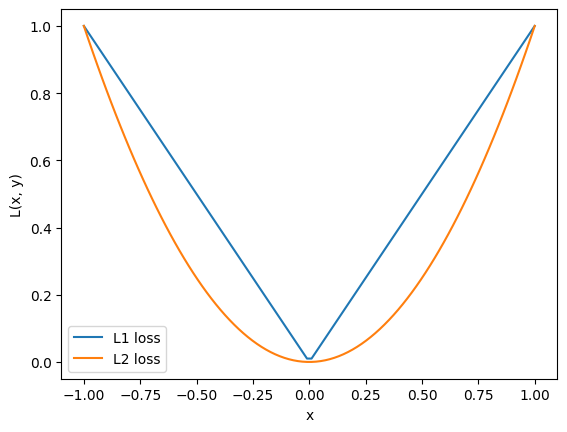
\includegraphics[width=0.4\linewidth]{Images/l1vsl2loss.png}
   \caption{L1 vs L2 loss values for a single data point. Ground truth $y$ is set to 0.}
   \label{fig:l1vsl2loss}
\end{figure}

\paragraph{Regularisation.} Training the model on the entire dataset can lead to overfitting. That is, the model's performance significantly decreases when tested on different data points. It occurs when the learned model becomes highly complex, no longer representing the overall data distribution but fitting to individual training samples instead. To make models generalise well to new data, we can add a regularisation term to the loss function. This term helps penalise the highly complex models, preventing overfitting. L1 ($\lambda \, \sum_i \abs{\theta_i}$) and L2 norm ($\lambda \, \sum_i \theta^2_i$) regularizations are two well-known terms. L1 norm pushes low parameter values to zero, encouraging sparsity. As some parameters become zero, L1 regularisation becomes highly effective in feature selection. L2 regularisation reduces model complexity but maintains the features. It manages multicollinearity by distributing the importance among correlated features and offers smooth solutions. The coefficient $\lambda$ defines the strength of the regularisation. If we combine a MSE with L2 regularisation, we will have the following loss function:

\begin{equation}
\mathcal{L}(\theta) = \frac{1}{m} \sum_{i=1}^{m} (y_i - f_\theta(x_i))^2 + \lambda \sum_{j=1}^{n} \theta_j^2
\label{MSE-with-L2reg}
\end{equation}

Here, $m$ is the number of training samples, and $n$ indicates the number of parameters. In HyperBRDF, I benefitted from L2 regularization for both latent representations and model parameters to maintain the features while reducing collinearity.

\paragraph{Data augmentation} is the process of producing altered versions of pre-existing data samples with the aim of increasing the diversity in the training dataset. Data augmentation is another strategy to prevent overfitting and make the model more generalizable to new samples. It also helps compensate for data-scarce regimes where collecting a large-scale dataset is highly impractical. The augmentation approach depends on the type of data. For images, the types of augmentation can include geometric transformations, such as rotating, scaling, translation, flipping, and cropping; colour space transformation, such as brightness, contrast, saturation and hue adjustment; noise injection; applying kernel filters; etc. In one-shot detail retouching, I extracted patches of size $3 \times 3$ with a stride of 1, which led to overlapping patches as a means of data augmentation.

\subsection{Multilayer Perceptrons}

Inspired by biological neural networks, deep neural networks (DNN) are designed as artificial neural networks that consist of layers, neurons, and connections between the neurons. As the ML field has advanced over time, the neural network models have become highly complex with multiple layers that lie between the input and output layers. To understand the basics of DNNs, consider a linear equation $y = \sum^n_i\vec{w_i} . \vec{x_i} + b = \vec{w}^T . \vec{x} + b$, where neurons are input data points $x_i$ that are connected to the output neuron $y$ via connections, known as weights $w_i$ (Figure \ref{fig:neuron}), and a bias term $b$. Here, we have the input layer (first layer with input neurons) and the output layer (last layer of the network)  and weights multiplied with input data points to obtain the output. This model can be considered a basic neural network architecture. 

\begin{wrapfigure}{r}{5cm}
  \centering
  % \fbox{\rule{0pt}{2in} \rule{0.9\linewidth}{0pt}}
   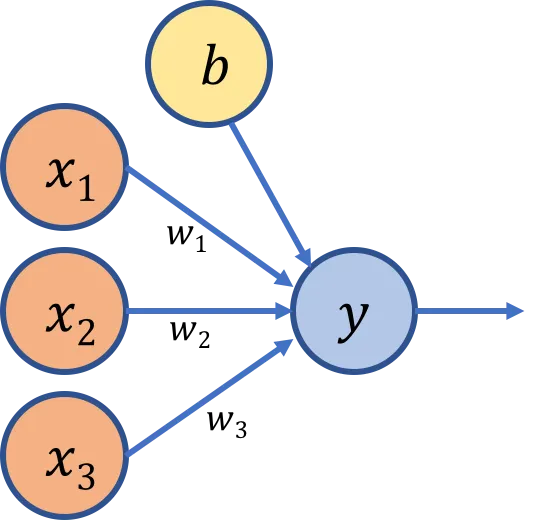
\includegraphics[width=\linewidth]{Images/neuron.png}
   \caption{Graph representation of a linear equation. Figure from [Issac, 2018].}
   \label{fig:neuron}
\end{wrapfigure}

The machine learning bit of neural networks is known as deep learning, a subfield of ML in which the learning process discussed above is used to learn the weights and biases of this equation or, more generally, the neural network. I mentioned earlier that nonlinearity is an inherent feature of deep learning. This comes from an additional function, known as the activation function, applied to the linear equation above ($y = \sigma(\vec{w} ^T. \vec{x} + b)$). The nonlinearity helps bring additional information to the linear system, which, otherwise, could have infinitely many solutions in the linear space.


With the assumption of a feedforward structure, a neural network can put its neurons into stacks of layers, each layer only depending on the previous layers. This model, a \textbf{multilayer perceptron (\gls{MLP})} (Figure \ref{fig:mlp}), is one of the simplest and most widely used neural network models that can be employed for multiple applications, such as image classification, regression, and pattern recognition. By extending the equation above, an MLP layer can be expressed in the matrix form as:
\begin{equation}
\vec{y} = \sigma \biggl(\mathbf{W}\vec{x} + \vec{b} \biggr)
\end{equation}
where $\mathbf{W}$ and $\vec{b}$ are the weight matrix and bias vector of the corresponding MLP layer. We can stack multiple such layers (hidden or intermediate layers) between the input and output layers, which increases the \textbf{depth} of the MLP:
\begin{equation}
\vec{y} = \sigma_2 \biggl( \mathbf{W}_2\sigma_1 \biggl(\mathbf{W}_1\vec{x} + \vec{b}_1 \biggr) + \vec{b}_2\biggr) 
\end{equation}
Here, each layer has its own weights and biases, weights multiplied by the output of the previous layer. We can compute the total number of parameters by multiplying the number of input and output neurons for each layer and then adding them all together along with the bias terms. 

%For instance, the total number of parameters in the MLP model shown below is $4 \times 5 + 5 \times 3 + 3 \times 2 + 5 + 3 + 2$.


\begin{figure}[ht]
  \centering
  % \fbox{\rule{0pt}{2in} \rule{0.9\linewidth}{0pt}}
   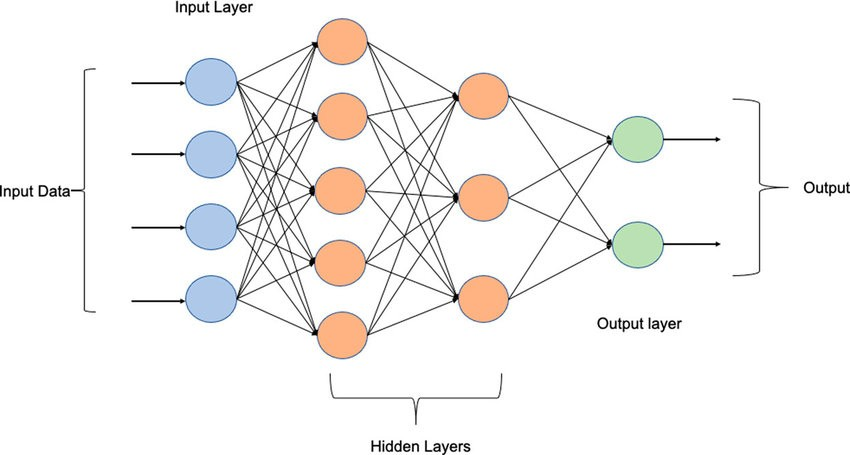
\includegraphics[width=0.8\linewidth]{Images/MLP.jpeg}
   \caption{A basic multilayer perceptron model. Figure from [Kishore NG, 2023].}
   \label{fig:mlp}
\end{figure}

The passing of the input towards the network to obtain the output is called \textbf{forward pass} or \textbf{forward propagation}. The \textbf{backward pass}, on the other hand, defines the training process of neural networks. Training in deep learning follows the same steps as discussed earlier for the ML model training. We compute a loss function based on the output obtained with the forward pass, then take its gradients to update the parameters (weights and biases in this case). As deep neural networks have multiple layers, computing the gradient of the loss with respect to the first layers requires applying the chain rule. The gradients propagate back towards the input. That is why backward pass is also called \textbf{backpropagation}. One problem with backpropagation is that the gradients can get extremely small as they backpropagate towards the input layer, known as \textbf{vanishing gradients}. It happens because the gradient with respect to early layers is the product of the gradient with respect to later layers. If the gradient in the last layers is smaller than one, their products vanish rapidly. ReLU activation function, batch normalization, skip connections and gradient scaling are methods to overcome the vanishing gradients problems.

\paragraph{Activation functions.} The choice of activation functions depends on the task and output expectations. The ones I utilised for this dissertation are as follows:

\begin{itemize}
\item The rectified linear function (ReLU):

\begin{equation}
\sigma(x) = max(x, 0)
\end{equation}

ReLU is one of the most commonly used activation functions in computer vision problems due to the lack of vanishing gradients and computational efficiency. It is also an ideal choice when the output values should not go below zero. For instance, the value range of image pixels is, in general, $[0, 1]$ after pre-processing, or the BRDF values should hold positivity.

\item The exponential linear unit (ELU):
\begin{equation}
 \sigma(x) = \begin{cases}
x, & \text{if $x>0$}\\
\exp(x) - 1,  & \text{if $x\leq0$} 
  \end{cases}
\end{equation}

\item Sinusoidal Activation Function:

\begin{equation}
\sigma(x) = \sin(x)
\label{eq:sine-act}
\end{equation}
\end{itemize}

\subsection{Neural implicit representations}

At the beginning of this chapter, I discussed the limitations of the image display and representation due to discretization. The real world is in a continuous spectrum, including geometry, light, reflectivity, and sound. However, we should discretise the inherently continuous signals for virtual representations and storage in computers. For example, images are represented as a grid of pixels, geometry as point clouds or meshes, and sound waves and electrical signals as discrete samples. The discrete representation bounds the amount of information about a signal to a discrete structure of a certain size. Not only scaling up an image does not bring any additional information but also causes artifacts, such as blurring or aliasing. 

To represent signals in a continuous domain, imagine we have a continuous function $f$ that maps the coordinates or locations to corresponding signal values. In an image case, the function $f$ takes $(x, y)$ pixel coordinates as input and outputs the corresponding RGB pixel value. This representation allows us to sample pixel grids at any resolution. More generally, the parameterisation of a signal as a mathematical formula offers a mapping from the coordinate space to the value space without resolution limitations. The difficulty with such a representation is to find the appropriate function since most signals are usually too complex to be analytically tractable. Neural implicit representations address this by representing signals with neural networks as they are essentially universal function approximators \cite{cybenko1989approximation}.

Recent advancements in computer vision and graphics research have transitioned from discrete representations to continuous function representations parameterised by multilayer perceptrons. These MLPs, also referred to as "coordinate-based" MLPs, utilise low-dimensional coordinates as inputs and are trained to output representations of shape, density, and/or colour at each respective input location \cite{ffn}. Their highly efficient compactness compared to grid-sampled representations as well as suitability for gradient-based optimisation make coordinate-based MLPs ideal for neural representations of signals. These MLPs have been employed to represent images \cite{nguyen2015deep}, volume density \cite{mildenhall2021nerf}, signed distance functions \cite{park2019deepsdf}, and BRDFs \cite{sztrajman2021neural}, achieving state-of-the-art performance across a range of tasks including shape and appearance representation, texture synthesis, and novel view synthesis.

It is worth mentioning that ReLU-based MLPs are known to have a spectral bias \cite{rahaman2019spectral}. That is, they struggle with predicting high-frequency components, mainly fitting to low-frequency ones. This spectral bias causes losses in details, and consequently, the represented signals become blurry. To enhance the capacity of MLPs for highly accurate representations, methods based on sinusoidal functions have been proposed. In NeRF, a positional encoding with $cos$ and $sin$ mapping is applied to the continuous 5D coordinates (spatial location $(x, y, z)$ and viewing direction $(\theta, \phi)$) before feeding them to the network for novel view synthesis. \citeauthor{ffn} \cite{ffn} later shows that positional encoding is a special case of Fourier features \cite{rahimi2007random} and proposes a more general mapping formula that can be applied across a range of different tasks, including image and 3D shape regression and MRI reconstruction. Along this line, \citeauthor{sitzmann2020siren} \cite{sitzmann2020siren} propose replacing ReLU activation functions with a sinusoidal one (Eqn. \ref{eq:sine-act}).

Fourier feature mapping function $\gamma$ maps input points $\mathbf{v}$ to a higher dimensional space with a set of sinusoid:
\begin{equation}
\gamma(v) = [\alpha_1 \cos(2 \, \pi \, \mathbf{b}^T_1 \, \mathbf{v}), \alpha_1 \sin(2 \, \pi \, \mathbf{b}^T_1 \, \mathbf{v}), ..., \alpha_1 \cos(n \, \pi \, \mathbf{b}^T_n \, \mathbf{v}), \alpha_1 \sin(n \, \pi \, \mathbf{b}^T_n \, \mathbf{v})]
\label{eq:ffn}
\end{equation}

where $b_i$ and $a_i$ are considered as  the Fourier basis frequencies and the corresponding Fourier series coefficients, respectively.

\begin{figure}[ht]
  \centering
  % \fbox{\rule{0pt}{2in} \rule{0.9\linewidth}{0pt}}
   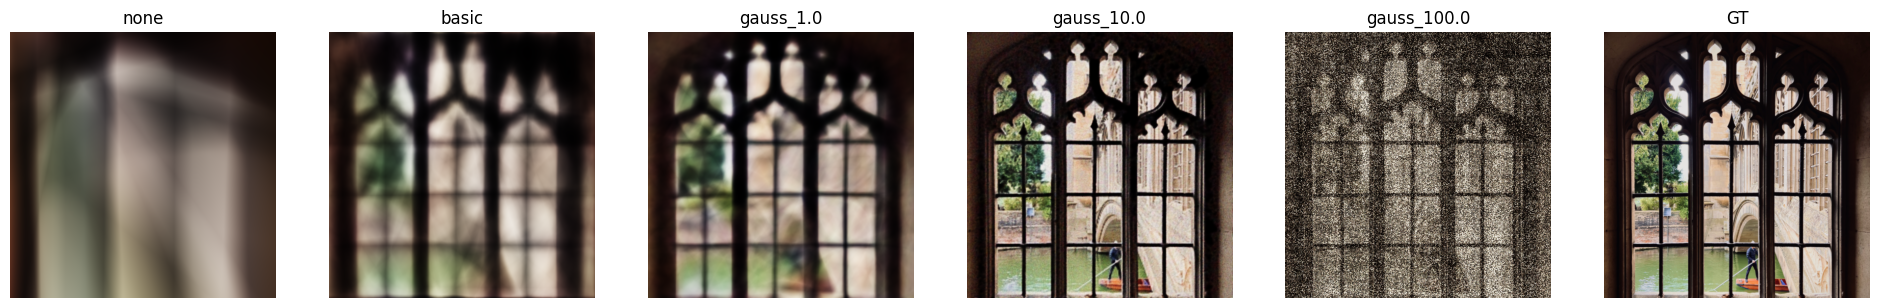
\includegraphics[width=\linewidth]{Images/FFN.png}
   \caption{To overcome the spectral bias in coordinate-based MLPs, a Fourier feature mapping \cite{ffn} can be applied before feeding the input to the model. Here, 'none' represents an MLP model without mapping. 'basic' and 'gauss' are different variants of Fourier feature maps, and 'GT' is the ground truth.}
   \label{fig:ffn}
\end{figure}

The effectiveness of the coordinate-based MLP models with periodic functions either as an activation or a mapping is compelling. However, the drawback of such neural representations is that they are designed for reconstruction of individual signals, causing overfitting. Therefore, I refrain from using such alternatives for the generalizable BRDF representation (HyperBRDF) and maintain a plain MLP model with ReLU activation functions.

\subsection{Diffusion models}